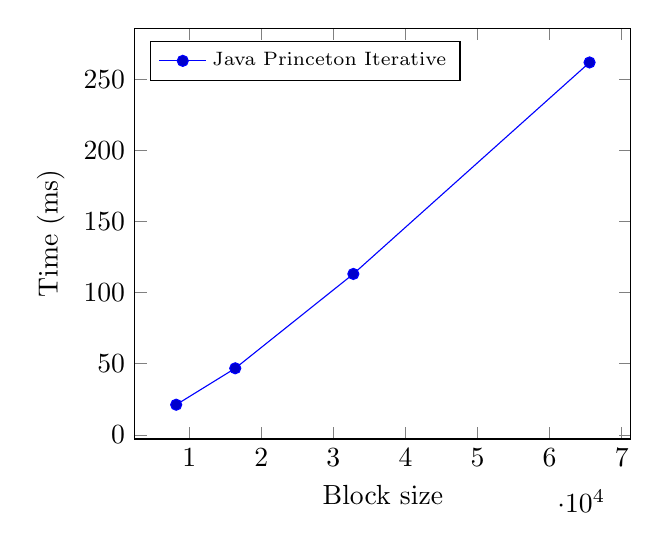
\begin{tikzpicture}
\begin{axis}[xlabel={Block size},ylabel={Time (ms)},width=0.65\linewidth,legend pos=north west,scaled y ticks = false,legend cell align=left,legend style={font=\scriptsize}]
\addplot coordinates {
(8192, 21.1757)
(16384, 46.8150)
(32768, 113.1953)
(65536, 261.9954)
};
\legend{Java Princeton Iterative}
\end{axis}
\end{tikzpicture}
